\documentclass{article}
\usepackage{epsfig}
\begin{document}
\title{Gentle Introduction to Python}
\author{Tom Kuiper}
\date{\today}

\maketitle

\section{Introduction}

Python is a  very elegant, syntactically simple scripting language.  However,
it has, in some circles, a reputation for being obscure.  Indeed, code written
by a computer science graduate may be almost unreadable by someone whose
background is in procedural languages like C, FORTRAN, IDL, Visual Basic, etc.
Nevertheless, Python can be used as a procedural language.  In time, one can
grow into the more sophisticated features.

\section{Python Basics}

\begin{figure}[h!tb]
\begin{center}
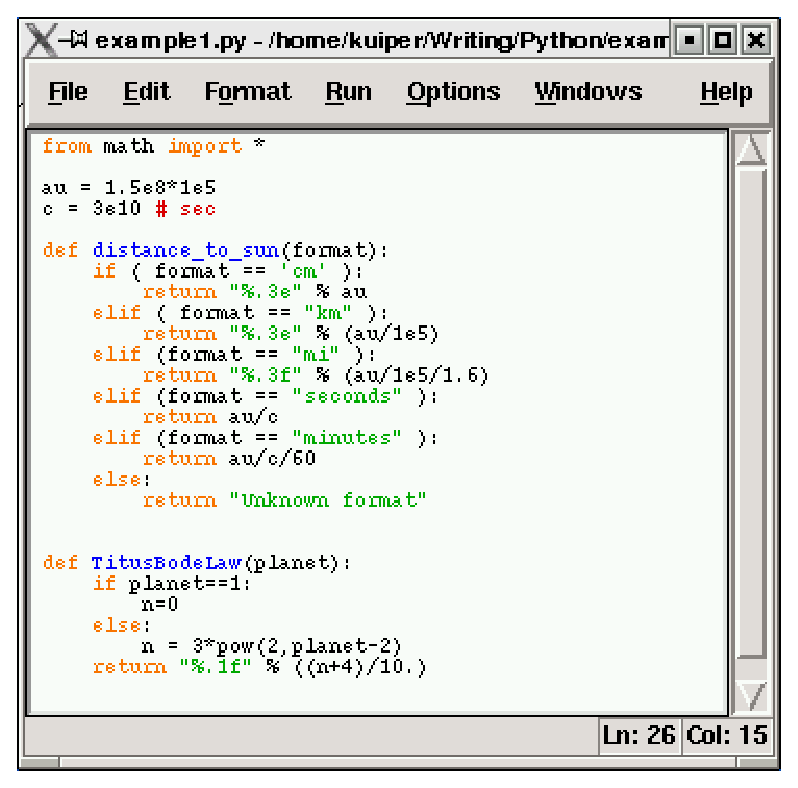
\epsfig{file=example1mod.ps,width=4in}
\caption{\label{fig:ex1_module}Two sample Python functions. (The height of
the window was adjusted to remove blank space.)}
\end{center}
\end{figure}

\subsection{A Simple Introduction}

The functions given in Figure~\ref{fig:ex1_module} should be easily
understood by anyone with some programming experience.
The points to note in {\ttfamily distance\_to\_sun()} are
\begin{enumerate}
\item Python only uses functions. (If Python functions are created from C or
FORTRAN, then subroutines are converted to functions, that is, the modified
arguments are returned as output.)
\item The type of a variable is implicit in the value it is assigned. The
variables {\ttfamily au} and {\ttfamily c} are type {\ttfamily float}. 
{\ttfamily format} is type {\ttfamily string}. There are ways to create
variables of one type from another type. For example {\ttfamily "\%.3e" \%
(au/1e5)} converts a {\ttfamily float} to a {\ttfamily string}.
\item The start of a block of code is indicated by a colon and any decent
editor, knowing that it is working on a {\ttfamily .py} file, will
automatically indent the next line.
\item A block of code ends with a return to the previous level of indentation.
Some keywords, like {\ttfamily return}, by definition end a block and the editor
will revert to the previous level.
\item Output formatting is a little odd but very similar to C except that
{\ttfamily \%} separates the format string from the list of variables to be
formatted, separated by commas and enclosed with parentheses.
\end{enumerate}

\subsection{Trying it out with Idle}

{\ttfamily idle} is a programming environment bundled with Python.  Start
{\ttfamily idle}, open a new window from the {\ttfamily File} menu.
You will then have the window shown in Figure~\ref{fig:ex1_module}.
Type in the code for {\ttfamily distance\_to\_sun()}, save it and run it.
{\ttfamily Run} is on the menu bar. In this case, Run produces no output.
It only defines the variables {\ttfamily au} and {\ttfamily c} and the
functions {\ttfamily distance\_to\_sun()} and {\ttfamily TitusBodeLaw()}.

In the {\ttfamily idle} main window (Figure~\ref{fig:ex1_idle_win}), verify
the function.
\begin{figure}[h!tb]
\begin{center}
\epsfig{file=example1idle.ps,width=5in}
\caption{\label{fig:ex1_idle_win}Test of the function shown in
Figure~\ref{fig:ex1_module}.}
\end{center}
\end{figure}
Note that the some of the outputs are strings while others are type
{\ttfamily float}. The strings can be converted back into  type
{\ttfamily float} by
\begin{verbatim}
>>> float('1.500e+08')
150000000.
\end{verbatim}

The above also illustrates that the Idle main window provides a Python command input.
The Python command line can useful by itself for simple calculations.
\begin{verbatim}
myself@somehost:~$ python
Python 2.3.5 (#2, Oct 16 2006, 19:19:48)
[GCC 3.3.5 (Debian 1:3.3.5-13)] on linux2
Type "help", "copyright", "credits" or "license" for more information.
>>> year = 365.25*24*60*60
>>> print "%.5e sec" % year
3.15576e+07 sec
print "%.5e sec" % (year/pi)
1.00451e+07 sec
\end{verbatim}

\subsection{Lists}

Lists are a generalized version of C and FORTRAN arrays. The following behaves like
a C array (indexed from 0 to 9).
\begin{verbatim}
>>> distance = []
>>> for i in range(1,10):
	distance.append(TitusBodeLaw(i))

	
>>> print distance
['0.4', '0.7', '1.0', '1.6', '2.8', '5.2', '10.0', '19.6', '38.8']
>>> print distance[2]
1.0
\end{verbatim}
Things to note:
\begin{enumerate}
\item When using the command prompt, a colon automatically starts a block
which ends when two linefeeds are entered. The block is then executed.
\item {\ttfamily range(start,stop,interval)} function takes the place of the
{\ttfamily for start to stop by interval} construct in most languages.
The argument {\ttfamily stop} is required. The default for {\ttfamily start}
is 0. If a third argument is given, it is {\ttfamily step}.
\item In fact, {\ttfamily range()} produces a list.
\begin{verbatim}
>>> range(2,10,2)
[2, 4, 6, 8]
\end{verbatim}
Note that 10 is not in the list, which would not be consistent with indexing
from 0.
\item One might expect that adding an item to the end of a list could be
done with a function {\ttfamily append(mylist,item)}.  However, {\ttfamily
append} as a keyword might very well appear elsewhere in a large program with
a different
meaning.  The dot construct indicates that this {\ttfamily append} function
belongs to the list data type only\footnote{For those who intend to swim in
deeper waters, let's note here that
the {\itshape object} {\ttfamily mylist} is an {\itshape instance} of the
{\itshape class} {\ttfamily list}. {\ttfamily mylist.append()} is a {\itshape
method} of the class {\ttfamily list}}.
\end{enumerate}

Lists can be very general, in that each item can be any kind of variable,
even another list. For example,
\begin{verbatim}
>>> Mercury = [0.39,[2439,2439],0.05527,58.6462,'']
>>> Venus = [0.72,[6051,6051],0.81499,243.01,'Cytherian']
>>> Earth = [1.00,[6378.140,6356,775],1.00,0.99726966,'Terrestrial']
\end{verbatim}
Of course, this is not the clearest way of encoding this information, since the
program has to know the meaning of the variable in each place in the list.

\subsection{Dictionaries}

Dictionaries are a much better way to encode diverse information. Consider
this:
\begin{verbatim}
>>> Mercury = {'au':0.39,'radii':[2439,2439],'mass':0.05527, 
... 'sid.rot.pd':58.6462,'genetive':''}
>>> Mercury.keys()
['mass', 'radii', 'au', 'genetive', 'sid.rot.pd']
\end{verbatim}

\begin{enumerate}
\item Python will give a continuation prompt of "..." when an input is
incomplete.
\item The data typei ({\itshape class}) {\ttfamily dictionary} has a
function ({\itshape method}) {\ttfamily keys}
which can be quite useful to see what data are defined in the dictionary.
\end{enumerate}

\subsection{Tuples}

A tuple is another {\itshape sequence} data type.
\begin{verbatim}
>>> ra = (5+(32+47.0/60)/60)*pi/12
>>> dec = -(5+(24+28.0/60)/60)*pi/180
>>> x = cos(ra)*cos(dec)
>>> y = sin(ra)*cos(dec)
>>> z = sin(dec)
>>> vector = x,y,z
>>> print vector
(0.11794886238916301, 0.98853742292222613, -0.094243457828042942)
\end{verbatim}
You can't change the items of a tuple (well, you can in a complicated way) but
unpacks more cleanly than a list.
\begin{verbatim}
>>> vector[1] = 5
Traceback (most recent call last):
  File "<stdin>", line 1, in ?
TypeError: object doesn't support item assignment
>>> d1,d2,d3 = vector
>>> print d2
0.988537422922
\end{verbatim} 
This suggests that in some cases it may be
convenient to have a function return a tuple:
\begin{verbatim}
>>> def direction_cosines(ra,dec):
...     x = cos(ra)*cos(dec)
...     y = sin(ra)*cos(dec)
...     z = sin(dec)
...     return x,y,z
...
>>> d1,d2,d3 = direction_cosines((5+(32+47.0/60)/60)*pi/12,\
                                -(5+(24+28.0/60)/60)*pi/180)
(0.11794886238916301, 0.98853742292222613, -0.094243457828042942)
\end{verbatim}

\section{Modules}

Modules group functions (and classes) by topic, such as numerical methods,
graphics, scientific disciplines, etc.  There are differen ways to access
functions that are in modules.

\subsection{Importing Code from Modules}

\subsubsection{{\ttfamily from {\itshape module} import *}}

In the example in Figure~\ref{fig:ex1_module} we passed over a key statement:
\begin{verbatim}
from math import *
\end{verbatim}
{\ttfamily math} is a module that provides the basic mathematical functions.
In this example, all the data and functions in {\ttfamily math} were brought into
current context, which may be that of the main command line or another module.
In fact, the code shown in Figure~\ref{fig:ex1_module} belongs implicitly to a
module called {\ttfamily example1} because it was saved in a file 
{\ttfamily example1.py}.

\subsubsection{The Search Path}

The {\ttfamily import} command searches all the directories
included in {\ttfamily sys.path} starting with the current directory.
\begin{verbatim}
>>> import sys
>>> print sys.path
['', '/usr/lib/python23.zip', '/usr/lib/python2.3',\
 '/usr/lib/python2.3/plat-linux2', '/usr/lib/python2.3/lib-tk',\
 '/usr/lib/python2.3/lib-dynload',\
 '/usr/local/lib/python2.3/site-packages',
 '/usr/lib/python2.3/site-packages',\
 '/usr/lib/python2.3/site-packages/HTMLgen',\
 '/usr/lib/python2.3/site-packages/Numeric',\
 '/usr/lib/python2.3/site-packages/PIL',\
 '/usr/lib/python2.3/site-packages/gtk-2.0']
\end{verbatim}
The path can be expanded by setting the environment variable {\ttfamily PYTHONPATH}
using the colon-separated syntax of {\ttfamily PATH}. These directories are
inserted between the current directory and the standard search path.
\begin{verbatim}
kuiper@nutmeg:~$ export PYTHONPATH=/home/kuiper:/home/kuiper:tmp
kuiper@nutmeg:~$ python
Python 2.3.5 (#2, Oct 16 2006, 19:19:48)
[GCC 3.3.5 (Debian 1:3.3.5-13)] on linux2
Type "help", "copyright", "credits" or "license" for more information.
>>> import sys
>>> print sys.path
['', '/home/kuiper', '/home/kuiper/tmp', '/usr/lib/python23.zip',\
 '/usr/lib/python2.3', '/usr/lib/python2.3/plat-linux2',
 ....
]
\end{verbatim}

\subsubsection{{\ttfamily import {\itshape module}}}

Another way to import data and functions from module would be as shown
here.
\begin{verbatim}
kuiper@nutmeg:~$ python
Python 2.3.5 (#2, Oct 16 2006, 19:19:48)
[GCC 3.3.5 (Debian 1:3.3.5-13)] on linux2
Type "help", "copyright", "credits" or "license" for more information.
>>> import math
>>> dir(math)
['__doc__', '__file__', '__name__', 'acos', 'asin', 'atan', 'atan2',\
 'ceil', 'cos', 'cosh', 'degrees', 'e', 'exp', 'fabs', 'floor',\
 'fmod', 'frexp', 'hypot', 'ldexp', 'log', 'log10', 'modf', 'pi',\
 'pow', 'radians', 'sin', 'sinh', 'sqrt', 'tan', 'tanh']
\end{verbatim}
(Note the useful {\ttfamily dir()} funsction.)
In this case, the module becomes accessible but not as an integral part of the
current environment. 
  This would be useful if one needed to have other
definitions for {\ttfamily e} and {\ttfamily pi}.
\begin{verbatim}
>>> e = 1.6e-19 \# coulomb
>>> pi = 8.8 \# parallax
>>> print math.pi
3.14159265359
>>> print math.e
2.71828182846
\end{verbatim}

\subsubsection{{\ttfamily}import {\itshape package} as {\itshape alias}}

If a package has a long name, it could be tedious to use the whole name every time.
In that case, the following may be more convenient:
\begin{verbatim}
>>> import datetime as D
>>> dir(D)
['MAXYEAR', 'MINYEAR', '__doc__', '__file__', '__name__', 'date',\
 'datetime', 'time', 'timedelta', 'tzinfo']
>>> print D.date.today()
2007-06-02
\end{verbatim}
This aliases the module {\ttfamily datetime} to {\ttfamily D}.

\subsection{Foreign Modules and OO Programming}

If you write all your own code, Python does not prevent you keeping to your
procedural programming habits.  However, there are very many useful Python
modules which are either built-in or are contributed by other programmers.
Almost invariably they are written in the object-oriented paradigm. The built-in
{\ttfamily datetime} module is a good example.  The last command in the
above example means, ``Print the result of invoking {\itshape method}
{\ttfamily today} of the (object) {\itshape class} {\ttfamily date} in the
module {\ttfamily D}.''

To the procedural programmer, the information available from the help function
is so obscure as to be almost useless. However, we now know from the above
example
that there are object classes called {\ttfamily date}, {\ttfamily datetime},
etc. in the {\ttfamily datetime} module. 
A class is a prototype object. In FORTRAN we might think of {\ttfamily
double} as a class and {\ttfamily pi} as an object which is an instance of
that class.

We can scan the help on the class {\ttfamily date} to discover that it has a 
method {\ttfamily today}. Below we create an object {\ttfamily d1} of the
class {\ttfamily date} in module {\ttfamily D (= datetime)} and invoke its
method {\ttfamily today()}.
\begin{verbatim}
>>> d1 = D.date
>>> d1.today()
datetime.date(2007, 6, 2)
>>> print d1.today()
2007-06-02
\end{verbatim}
Now we create an object obtained obtained from the method {\ttfamily today}
and invoke some of its methods.
\begin{verbatim}
td = d1.today()
>>> print td
2007-06-02
>>> td.weekday()
5
>>> td.isoweekday()
6
>>> td.isocalendar()
(2007, 22, 6)
>>> td.isoformat()
'2007-06-02'
>>> td.ctime()
'Sat Jun  2 00:00:00 2007'
\end{verbatim}
{\ttfamily isocalendar()} returns the year, week number, and day of the week
from object {\ttfamily td}.
In the case of method {\ttfamily ctime}, the time is 00:00:00 because
{\ttfamily td} is a {\ttfamily date}
object instead of a {\ttfamily datetime} object.

We can obtain {\itshape attributes} of the {\itshape object} {\ttfamily td}:
\begin{verbatim}
>>> td.year
2007
>>> td.month
6
>>> td.day
2
\end{verbatim}
With these clues, the goobledygook returned from
\begin{verbatim}
>>> help(D.date)
\end{verbatim}
begins to make some sense.  Remember that you can always try something quickly
at the command prompt.

\section{Help}

There is, as part of the documentation of thePython distribution, a Global Module Index.
That would be the place to start looking for a module name that suggests that it may
have what you need for some task.

Clicking on {\ttfamily datetime} brings up the Python Library Reference page on
this module. On a Linux system it would be found at\newline
{\ttfamily /usr/share/doc/python/html/lib/module-datetime.html}. The information
here is definitely clearer than what the function {\ttfamily help()}
provides.

For your own code, it is certainly less effort to provide good help information.
\begin{figure}[h!tb]
\begin{center}
\epsfig{file=example1help.ps,width=4in}
\caption{\label{fig:ex1help}The module shown in Figure~\ref{fig:ex1_module}
with documentation added.}
\end{center}
\end{figure}
Figure~\ref{fig:ex1help} shows the module {\ttfamily example1} with
{\ttfamily help} documentation added. Your documentation will now be
available.
\begin{verbatim}
Help on module example1:

NAME
    example1

FILE
    /home/kuiper/Writing/Python/example1.py

DESCRIPTION
    This module defines the constants
    au - in cm
    c  - the speed of light in cm/s
    and the functions
    distance_to_sun(format)
    TitusBodeLaw(planet_number)

FUNCTIONS
    TitusBodeLaw(planet)
        Given a planet number, starting with 1 for
        Mercury, it returns the orbital radius as
        calulated by the Titus-Bode Law

    acos(...)
        acos(x)

        Return the arc cosine (measured in radians) of x.
....
    distance_to_sun(format)
        Given a format (or unit) this returns thw
        mean distance of the sun in that unit
....
DATA
    au = 15000000000000.0
    c = 30000000000.0
    e = 2.7182818284590451
    pi = 3.1415926535897931

>>> help(example1.distance_to_sun)
Help on function distance_to_sun in module example1:

distance_to_sun(format)
    Given a format (or unit) this returns thw
    mean distance of the sun in that unit
\end{verbatim}
Notice that the {\ttfamily math} functions are part of {\ttfamily example1}
because of the form of the {\ttfamily import} used. In the case of the
{\ttfamily math} package, this is generally safe since the function names
are almost universally reserved for mathematical operations.

\section{Organizing Code}

\subsection{Nesting Modules}

Back to your own programming.  Let's imagine that you have the module
{\ttfamily jplephem} from Rick Fisher at NRAO.  You compiled a module
{\ttfamily coco} from FORTRAN sources by Wallace of the Starlink project
using {\ttfamily pyfort},
and you have some of your own Python astronomy procedures in a module
{\ttfamily astro}. You can include everything in  {\ttfamily jplephem} and
{\ttfamily coco} as part of your module {\ttfamily astro} by putting
in the latter
\begin{verbatim}
import jplephem
import coco
\end{verbatim}
If you import {\ttfamily astro} and do a {\ttfamily dir{}} you will see
the contents of all the modules, as well as some others such as
{\ttfamily math} and {\ttfamily Numeric}.

\subsection{Packages}

\appendix

\section{Module {\ttfamily Gnuplot}}

The module {\ttfamily Gnuplot} provides an interface to the {\ttfamily gnuplot}
program, which must be installed on the system.

\subsection{Class {\ttfamily Gnuplot}}

A plotting session (there can be several simultaneously) is an instance of the
class {\ttfamily Gnuplot}.  The same name is used for the module and the class.
For this reason, do not use {\ttfamily from Gnuplot import *}.
Here is an example:
\begin{verbatim}
>>> import Gnuplot
>>> g1 = Gnuplot.Gnuplot()
>>> g2 = Gnuplot.Gnuplot()
\end{verbatim}
We now have two plot objects.  Any valid {\ttfamily gnuplot} command can be passed
to such objects.
\begin{verbatim}
>>> g1('set xrange [-100:100])
>>> g1('set pointsize 2')
\end{verbatim}
The objects can have attributes, such as a title.
\begin{verbatim}
g1.title('Graph 1')
\end{verbatim}

\subsection{Class {\ttfamily PlotItem}}

A {\ttfamily Gnuplot} object knows how to plot one or more
{\ttfamily PlotItem} objects.
There are methods to create various types of such objects.
\begin{verbatim}
>>> import Numeric
>>> x = arange(10, typecode='fd')
>>> y1 = x**2
>>> p1 = Gnuplot.Data(x,y1,title='x^2')
>>> p2 = Gnuplot.Func('x**2')
>>> p3 = Gnuplot.Data([[0.5,0.25],[1.5,2.25],[2.5,6.25],\
                       [3.5,12.25]],title='more data')
>>> p4 = Gnuplot.File('gnuplot_ex1.dat')
>>> g.xlabel('x')
>>> g.ylabel('y')
>>> g.plot(p1,p2,p3,p4)
\end{verbatim}
\begin{figure}[h!tb]
\begin{center}
\epsfig{file=gnuplot_ex1.ps,width=5in}
\caption{\label{fig:gnuplot1}An example of the use of the {\ttfamily Gnuplot}
module.  See Appendix~\ref{ap:random} for how the data in the file were generated.}
\end{center}
\end{figure}

There is one other type of {\ttfamily PlotItem}, which is generated by
function {\ttfamily GridData}. The arguments are, in this order, a two-dimensional
data array with dimensions ({\ttfamily Nx,Ny}), an one-dimensional array
of corresponding {\ttfamily x}-values, and a similar array of {\ttfamily x}-values.
There are other, optional arguments identified with keywords, like the keyword
{\ttfamily title} in the above example.

\section{Module {\ttfamily random}}\label{ap:random}

This illustrates the use of the {\ttfamily random}.
\begin{verbatim}
#!/usr/bin/python

import math
import random

for i in range(10):
    x = 9*random.random()
    y = pow(x+random.gauss(0,0.3),2)
    print x,y
\end{verbatim}
It also shows how to create an executable Python script.  The data file was created
with
\begin{verbatim}
./gnuplot_ex1a.py > gnuplot_ex1.dat
\end{verbatim}

\subsection{Functions}

These are the same as the methods of the class {\ttfamily Random} (see below).
Basically,
they can be invoked without creating an object.
\begin{verbatim}
>>> random.randint(9,19)
15
\end{verbatim}
For people who want to give object-oriented programming as wide a berth as
possible, this may be the best way to go.
The documentation obtained from
\begin{verbatim}
>>> help(random)
\end{verbatim}
gives all the functions after the definitions of the classes, and is pretty clear.
Ignore the first
argument {\ttfamily self}.  Arguments with defaults show the default value
after an equal sign.

\subsection{Classes}

\subsubsection{{\ttfamily Random}}

This is the base random number generator with, among others,
 the following methods:
\begin{description}
\item{{\ttfamily random()}}
      Return a float in the interval (0, 1).
\item{{\ttfamily seed(<optional>)}} Initialize internal state from hashable object.
\item{{\ttfamily gauss(nean, standard\_deviation)}}
\item{{\ttfamily randint(a, b)}}
      Return random integer in range [a, b], including both end points.
\item{{\ttfamily randrange(start, stop=None, step=1)}}
      Choose a random item from range(start, stop[, step]). In this case,
      follwing the Python convention, the endpoint is not includes.
\item{{\ttfamily uniform(a, b)}}
      Get a random number in the range [a, b).
\end{description}
and many more. The documentation obtained from
\begin{verbatim}
>>> help(random)
\end{verbatim}
gives all the methods and is pretty clear.

\subsubsection{Class {\ttfamily WichmannHill(Random)}}

This is a subclass of {\ttfamily Random}.
It's a different way of generating random numbers.  It has almost all the same
methods as {\ttfamily Random}.
\end{document}